\documentclass[CJK]{beamer}
%\usepackage{CJKutf8}
\usepackage{beamerthemesplit}
\usepackage{}
%\usetheme{Frankfurt}
%\usetheme{CambridgeUS}
%\usecolortheme{beaver}
%\usetheme{AnnArbor}
\usetheme{Dresden}
%\usebeamercolor{beetle}
\usepackage{xeCJK}
\setCJKmainfont{AR PL KaitiM GB}
%\useoutertheme{miniframes}
\usepackage{amsmath}
\usepackage{graphicx}
\usepackage{float} 
\usepackage{subfigure}
\usepackage{amssymb}
\usepackage{graphicx}
\usepackage{eufrak}
\usepackage{color}
\usepackage{array}
\usepackage{slashed}
\usepackage{simplewick}
\usepackage{tikz}
\usepackage{tcolorbox}
\usepackage[T1]{fontenc}
\graphicspath{{../figures/}}

%%figures
\def\lfig#1#2{\includegraphics[width=#1 in]{#2}}
\def\addfig#1#2{\begin{center}\includegraphics[width=#1 in]{#2}\end{center}}
\def\wulian{
\includegraphics[width=0.18in]{emoji_wulian.jpg}}
\def\bigwulian{
\includegraphics[width=0.35in]{emoji_wulian.jpg}}
\def\bye{
\includegraphics[width=0.18in]{emoji_bye.jpg}}
\def\bigbye{
\includegraphics[width=0.35in]{emoji_bye.jpg}}
\def\huaixiao{
\includegraphics[width=0.18in]{emoji_huaixiao.jpg}}
\def\bighuaixiao{
\includegraphics[width=0.35in]{emoji_huaixiao.jpg}}
\def\jianxiao{
\includegraphics[width=0.18in]{emoji_jianxiao.jpg}}
\def\bigjianxiao{
\includegraphics[width=0.35in]{emoji_jianxiao.jpg}}
%% colors
\def\blacktext#1{{\color{black}#1}}
\def\bluetext#1{{\color{blue}#1}}
\def\redtext#1{{\color{red}#1}}
\def\darkbluetext#1{{\color[rgb]{0,0.2,0.6}#1}}
\def\skybluetext#1{{\color[rgb]{0.2,0.7,1.}#1}}
\def\cyantext#1{{\color[rgb]{0.,0.5,0.5}#1}}
\def\greentext#1{{\color[rgb]{0,0.7,0.1}#1}}
\def\darkgray{\color[rgb]{0.2,0.2,0.2}}
\def\lightgray{\color[rgb]{0.6,0.6,0.6}}
\def\gray{\color[rgb]{0.4,0.4,0.4}}
\def\blue{\color{blue}}
\def\red{\color{red}}
\def\green{\color{green}}
\def\darkgreen{\color[rgb]{0,0.4,0.1}}
\def\darkblue{\color[rgb]{0,0.2,0.6}}
\def\skyblue{\color[rgb]{0.2,0.7,1.}}
%%control
\def\be{\begin{equation}}
\def\ee{\nonumber\end{equation}}
\def\bea{\begin{eqnarray*}}
\def\eea{\nonumber\end{eqnarray*}}
\def\bch{}
\def\ech{}
\def\bitem{\begin{itemize}}
\def\eitem{\end{itemize}}
\def\bcenter{\begin{center}}
\def\ecenter{\end{center}}
\def\bex{\begin{minipage}{0.2\textwidth}
\includegraphics[width=0.6in]{jugelizi.png}\end{minipage}\begin{minipage}{0.76\textwidth}}
\def\eex{\end{minipage}}
\def\chtitle#1{\frametitle{\bch#1\ech}}
\def\bmat#1{\left(\begin{array}{#1}}
\def\emat{\end{array}\right)}
\def\bcase#1{\left\{\begin{array}{#1}}
\def\ecase{\end{array}\right.}
\def\bmini#1{\begin{minipage}{#1\textwidth}}
\def\emini{\end{minipage}}
\def\tbox#1{\begin{tcolorbox}#1\end{tcolorbox}}
\def\pfrac#1#2#3{\left(\frac{\partial #1}{\partial #2}\right)_{#3}}
%%symbols
\def\bropt{\,(\ \ \ )}
\def\sone{$\star$}
\def\stwo{$\star\star$}
\def\sthree{$\star\star\star$}
\def\sfour{$\star\star\star\star$}
\def\sfive{$\star\star\star\star\star$}
\def\rint{{\int_\leftrightarrow}}
\def\roint{{\oint_\leftrightarrow}}
\def\stdHf{{\textit{\r H}_f}}
\def\deltaH{{\Delta \textit{\r H}}}
\def\ii{{\dot{\imath}}}
\def\skipline{{\vskip0.1in}}
\def\skiplines{{\vskip0.2in}}
\def\lagr{{\mathcal{L}}}
\def\hamil{{\mathcal{H}}}
\def\vecv{{\mathbf{v}}}
\def\vecx{{\mathbf{x}}}
\def\vecy{{\mathbf{y}}}
\def\veck{{\mathbf{k}}}
\def\vecp{{\mathbf{p}}}
\def\vecn{{\mathbf{n}}}
\def\vecA{{\mathbf{A}}}
\def\vecP{{\mathbf{P}}}
\def\vecsigma{{\mathbf{\sigma}}}
\def\hatJn{{\hat{J_\vecn}}}
\def\hatJx{{\hat{J_x}}}
\def\hatJy{{\hat{J_y}}}
\def\hatJz{{\hat{J_z}}}
\def\hatj#1{\hat{J_{#1}}}
\def\hatphi{{\hat{\phi}}}
\def\hatq{{\hat{q}}}
\def\hatpi{{\hat{\pi}}}
\def\vel{\upsilon}
\def\Dint{{\mathcal{D}}}
\def\adag{{\hat{a}^\dagger}}
\def\bdag{{\hat{b}^\dagger}}
\def\cdag{{\hat{c}^\dagger}}
\def\ddag{{\hat{d}^\dagger}}
\def\hata{{\hat{a}}}
\def\hatb{{\hat{b}}}
\def\hatc{{\hat{c}}}
\def\hatd{{\hat{d}}}
\def\hatN{{\hat{N}}}
\def\hatH{{\hat{H}}}
\def\hatp{{\hat{p}}}
\def\Fup{{F^{\mu\nu}}}
\def\Fdown{{F_{\mu\nu}}}
\def\newl{\nonumber \\}
\def\vece{\mathrm{e}}
\def\calM{{\mathcal{M}}}
\def\calT{{\mathcal{T}}}
\def\calR{{\mathcal{R}}}
\def\barpsi{\bar{\psi}}
\def\baru{\bar{u}}
\def\barv{\bar{\upsilon}}
\def\qeq{\stackrel{?}{=}}
\def\torder#1{\mathcal{T}\left(#1\right)}
\def\rorder#1{\mathcal{R}\left(#1\right)}
\def\contr#1#2{\contraction{}{#1}{}{#2}#1#2}
\def\trof#1{\mathrm{Tr}\left(#1\right)}
\def\trace{\mathrm{Tr}}
\def\comm#1{\ \ \ \left(\mathrm{used}\ #1\right)}
\def\tcomm#1{\ \ \ (\text{#1})}
\def\slp{\slashed{p}}
\def\slk{\slashed{k}}
\def\calp{{\mathfrak{p}}}
\def\veccalp{\mathbf{\mathfrak{p}}}
\def\Tthree{T_{\tiny \textcircled{3}}}
\def\pthree{p_{\tiny \textcircled{3}}}
\def\dbar{{\,\mathchar'26\mkern-12mu d}}
\def\erf{\mathrm{erf}}
\def\const{\mathrm{constant}}
\def\pheat{\pfrac p{\ln T}V}
\def\vheat{\pfrac V{\ln T}p}
%%units
\def\fdeg{{^\circ \mathrm{F}}}
\def\cdeg{^\circ \mathrm{C}}
\def\atm{\,\mathrm{atm}}
\def\angstrom{\,\text{\AA}}
\def\SIL{\,\mathrm{L}}
\def\SIkm{\,\mathrm{km}}
\def\SIyr{\,\mathrm{yr}}
\def\SIGyr{\,\mathrm{Gyr}}
\def\SIV{\,\mathrm{V}}
\def\SImV{\,\mathrm{mV}}
\def\SIeV{\,\mathrm{eV}}
\def\SIkeV{\,\mathrm{keV}}
\def\SIMeV{\,\mathrm{MeV}}
\def\SIGeV{\,\mathrm{GeV}}
\def\SIcal{\,\mathrm{cal}}
\def\SIkcal{\,\mathrm{kcal}}
\def\SImol{\,\mathrm{mol}}
\def\SIN{\,\mathrm{N}}
\def\SIHz{\,\mathrm{Hz}}
\def\SIm{\,\mathrm{m}}
\def\SIcm{\,\mathrm{cm}}
\def\SIfm{\,\mathrm{fm}}
\def\SImm{\,\mathrm{mm}}
\def\SInm{\,\mathrm{nm}}
\def\SImum{\,\mathrm{\mu m}}
\def\SIJ{\,\mathrm{J}}
\def\SIW{\,\mathrm{W}}
\def\SIkJ{\,\mathrm{kJ}}
\def\SIs{\,\mathrm{s}}
\def\SIkg{\,\mathrm{kg}}
\def\SIg{\,\mathrm{g}}
\def\SIK{\,\mathrm{K}}
\def\SImmHg{\,\mathrm{mmHg}}
\def\SIPa{\,\mathrm{Pa}}
\def\secpage#1#2{\begin{frame}\bch\bcenter{\bf \Huge #1} \skipline \tbox{\bcenter #2\ecenter}\ecenter\ech\end{frame}}

\usepackage{amssymb}
\newcommand{\field}{\mathscr{F}}

\newcommand{\reals}{\mathbb{R}}
\newcommand{\complexs}{\mathbb{C}}
\newcommand{\ints}{\mathbb{Z}}
%\newcommand{\dim}{\mathrm{dim\ }}
\newcommand{\diag}{\mathrm{diag \ }}
\newcommand{\up}{\uparrow}
\newcommand{\down}{\downarrow}
\newcommand{\su}{\mathfrak{su}}
\newcommand{\so}{\mathfrak{so}}
\newcommand{\tr}{\mathrm{tr\ }}
\newcommand{\card}{\mathrm{card \ }}

\newtheorem{thm}{定理}[section]
\newtheorem{axm}{公理}[section]
\newtheorem{dfn}{定义}[section]

%\cpic{<尺寸>}{<文件名>}}用于生成居中的图片。
\newcommand{\cpic}[2]{
\begin{center}
\includegraphics[scale=#1]{#2}
\end{center}
}

%\cpicn{<尺寸>}{<文件名>}{<注释>}用于生成居中且带有注释的图片,其label为图片名。
\newcommand{\cpicn}[3]
{
\begin{figure}[h!]
\cpic{#1}{#2}
\caption{#3\label{#2}}
\end{figure}
}

\title{Talk 5 Shine a light}
  \author{}
  \date{}


\begin{document}

\begin{frame}
 
\begin{center}
\begin{Large}
  \bch
  \begin{center}

\includegraphics[width = 1.2in]{whopper.jpg}
\end{center}

{\bf A}pplication of {\bf Q}uantum {\bf M}echanics

{\vskip 0.1in}

Talk 5-Shine a light

\ech
\end{Large}
\end{center}


\vskip 0.1in
\begin{center}
Haoting Xu
\vskip 0.1in
xuht9@mail2.sysu.edu.cn
\vskip 0.1in
{\tiny \url{https://github.com/HaotingXu/seminar_lec/shine_a_light} }\\
\end{center}


\end{frame}



\section{Introduction}
\begin{frame}
\frametitle{\bch高中物理的疑惑  \ech}
\bch
在高中物理选修3-5我们学过,如果使用光照射原子,如果光子的能量恰好为
\be
h\nu = E_2 - E_1
\ee
那么电子就会从状态1(可以是基态)跃迁到状态2(激发态)上。激发态不稳定,立刻又会落回基态,发出同样频率的光子。

But why?
\cpic{0.1}{3-5}
\ech
\end{frame}

\begin{frame}
\frametitle{\bch 原子物理的疑惑 \ech}
\bch
学过量子力学之后大家都知道,氢原子的一个状态是不同本征态之间的叠加(加上一个时间震荡因子)
\be
|\Psi\rangle = \sum_i c_i e ^{-iEt/\hbar}|\psi_i\rangle 
\ee
根据通常的量子力学,本征态不论是激发态还是基态都及其稳定,为何激发态会自发地向基态转变? 既然是不同本征态的叠加,何为跃迁?
\ech
\end{frame}
\begin{frame}
\frametitle{\bch跃迁的物理本质  \ech}
\bch
光的本质是电磁波,在这里我们先使用经典的处理方法,完整的处理需要将光场量子化(之后会提到)。对于单色光(平面波),有
\be
\vec{E} = \vec{E_0} e^{i(\vec{k}\cdot\vec{x}-\omega t)},\,\vec{B} = \frac{1}{c}(\hat{\vec{k}}\times \vec{E}_0)e^{i(\vec{k}\cdot\vec{x}-\omega t)}
\ee
其中角频率和波长
\be
\omega = c|\vec{k}|,\, \lambda = 2\pi c /\omega
\ee
\ech
\end{frame}
\begin{frame}\frametitle{\bch 对光子的条件\ech}
  \bch
  \begin{enumerate}[(1)]
  \item 光子的波长与\textbf{跃迁所需能量相近}
  \item 光的波长远远大于原子的尺度 $\lambda >> a_0$,所以电磁场可认为是空间均匀的
  \end{enumerate}
  上述两种条件是自洽的,典型的波长为$\lambda\simeq \frac{2\pi a_0}{\alpha},\,\alpha = 1/137$。
  \ech
\end{frame}

\begin{frame}\frametitle{\bch 电场vs磁场\ech}
  \bch
  斯塔克效应引起的能级分裂
  \be
  \Delta E \simeq \frac{e\varepsilon \hbar}{mc\alpha}
  \ee
  塞曼效应引起的能级分裂
  \be
  \Delta E \simeq \frac{eB\hbar}{2m} = \frac{e\varepsilon\hbar}{2mc}
  \ee
  电场引起的分裂大概是磁场的137倍,所以我们暂时不考虑磁场的效应。
  \ech
\end{frame}
\section{Rabi Oscillation}
\begin{frame}\frametitle{\bch哈密顿量 \ech}
  \bch
  带电粒子在电磁场中的哈密顿量为
  \be
  H = \frac{1}{2m}(\vec{p}+e\vec{A})^2 + q\phi
  \ee
  因为波长远大于玻尔半径,故电场可以看做是时变的。我们这里取$\vec{A} = 0, \, \phi = \vec{E}_0\cdot \vec{x}\cos(\omega t)$,电子总的哈密顿量可看成氢原子的哈密顿量加上微扰
  \be
  H = H_0 + \Delta H(t) = H_0 + e\vec{E_0}\cdot \vec{x} \cos(\omega t)
  \ee
  \ech
\end{frame}
\begin{frame}\frametitle{\bch含时微扰 \ech}
  \bch
  我们只考虑两个我们关注的态,$|\psi_1\rangle, |\psi_2\rangle$,没有电场的情况下,一般的态是他们俩的线性组合
  \be
  |\Psi (t)\rangle = c_1(t)e^{-iE_1t/\hbar}|\psi_1\rangle + c_2(t)e^{-iE_2t/\hbar}|\psi_2\rangle
  \ee
  其中$|c_1|^2+ |c_2|^2 = 1$,将上式带入含时薛定谔方程中
  \be
  i\hbar \frac{\partial|\Psi\rangle}{\partial t} = (H_0+\Delta H) |\Psi\rangle
  \ee
  得到的式子分别与$|\psi_1\rangle,|\psi_2\rangle$做内积,定义$\hbar \omega_0 = E_2-E_1$
  \be
  \left\{
  \begin{aligned}
    i\hbar \dot{c}_1(t) &=& c_1(t)\langle \psi_1|\Delta H|\psi_1\rangle+c_2(t)e^{-i\omega_0 t}\langle \psi_1|\Delta H|\psi_2\rangle \\
    i\hbar \dot{c}_2(t) &=& c_1(t)e^{i\omega_0 t}\langle \psi_2|\Delta H|\psi_1\rangle+c_2(t)\langle \psi_2|\Delta H|\psi_2\rangle \\
  \end{aligned}
  \right.
  \ee
  \ech
\end{frame}
\begin{frame}\frametitle{\bch 计算矩阵元\ech}
  \bch
  矩阵元为
  \be
  \langle \psi_i|\Delta H|\psi_j\rangle = e\vec{E}_0\cdot \langle\psi_i| \vec{x}|\psi_j\rangle\cos\omega t
  \ee
  $\vec{x}$是奇宇称算符
  \be
  \langle\psi_i | \vec{x}|\psi_j\rangle = -\langle\psi_i|\hat{\pi}\hat{\vec{x}}\hat{\pi}|\psi_j\rangle = (-1)^{p_i+p_j+1} \langle\psi_i | \vec{x}|\psi_j\rangle
  \ee
  故当两个态宇称相同时矩阵元为0,两个态宇称相反时矩阵元不为0。判断宇称用到氢原子波函数
  \be
  \psi = R(r) e^{im\phi} P_l^m(\cos\theta)
  \ee
  可见,如果$i=j$,矩阵元为0。两个态宇称相反时才能发生跃迁(选择定则)。
  \ech
\end{frame}
\begin{frame}\frametitle{\bch 拉比频率\ech}
  \bch
  说了这么多,我们得到很多态之间的矩阵元都为0。但是得到矩阵元的一般公式是困难的,反正它只是个常数,我们不妨定义拉比频率
  \be
  \hbar \Omega = e\vec{E}_0\langle\psi_1|\vec{x}|\psi_2\rangle
  \ee
  利用上面的定义和欧拉公式$e^{i\theta} = \cos\theta+i\sin\theta$,得到
  \be
  \left\{
  \begin{aligned}
    i\dot{c}_1&=&\frac{\Omega}{2}\left[e^{i(\omega - \omega_0)t}+e^{i(\omega+\omega_0)t}\right]c_2\\
    i\dot{c}_2&=&\frac{\Omega}{2}\left[e^{-i(\omega - \omega_0)t}+e^{i(\omega+\omega_0)t}\right]c_1
  \end{aligned}
  \right.
  \ee
  因为$\omega$十分接近$\omega_0$,所以$|\omega-\omega_0|<<\omega+\omega_0$,所以可见第二项振动的特别快,在时间平均的意义下可以忽略。这个近似叫做旋转波近似,叫这个名字是因为核磁共振(nuclear magnetic resonance)中有类似的处理方法。
  \ech
\end{frame}

\begin{frame} \frametitle{\bch 拉比共振\ech}
  \bch
  采取上述近似后,如果定义$\delta = \omega - \omega_0$,方程变为
  \be
  \left\{
  \begin{aligned}
    i\dot{c}_1 &=& \frac{\Omega}{2}e^{i\delta t}c_2 \\
    i\dot{c}_2 &=& \frac{\Omega}{2}e^{-i\delta t}c_1
  \end{aligned}
  \right.
  \ee
  现在我们考虑入射光频率恰好等于跃迁所需的频率,即$\delta = 0 $,这时方程变为
  \be
  \left\{
  \begin{aligned}
    i\dot{c}_1&=&\frac{\Omega}{2} c_2\\
    i\dot{c}_2&=& \frac{\Omega}{2}c_1
  \end{aligned}
  \right.
  \ee
  \ech
\end{frame}
\begin{frame}\frametitle{\bch 求解方程\ech}
  \bch
  取一个初始条件$c_1(0) = 1, \, c_2(0) = 0$,得到方程的解
  \be
  \left\{
  \begin{aligned}
    c_1 &=& \cos\left(\frac{\Omega t}{2}\right) \\
    c_2 &=& -i\sin\left(\frac{\Omega t}{2}\right)
  \end{aligned}
  \right.
  \ee
  计算取每个态的概率,得到
  \be
  \begin{aligned}
  P_1(t) &=& \cos^2\left(\frac{\Omega t}{2}\right)\\
  P_2(t) &=& \sin^2 \left(\frac{\Omega t}{2}\right)
  \end{aligned}
  \ee
  可见,状态1的概率和状态2的概率都在不断振动。
  \ech
\end{frame}
\begin{frame}\frametitle{\bch 拉比振动\ech}
  \bch
  将$P_1,P_2$画出图来如下图所示
  \begin{center}
    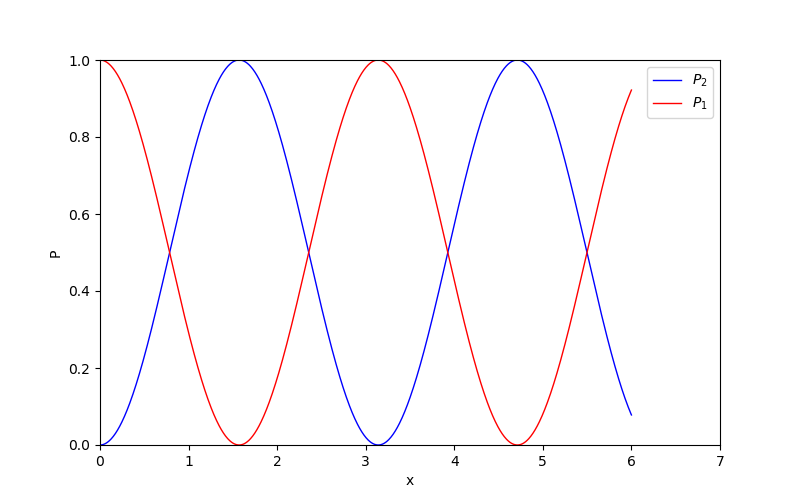
\includegraphics[width = 2.5in]{flopping}
  \end{center}
  这就叫做拉比振动(Rabi Oscillation or Rabi flopping)。振动周期为$\frac{2\pi}{\Omega}$,如果我们照射时间恰好等于$\frac{\pi}{\Omega}$,这之后立即停止照射,就会恰好得到一个激发态。但如果我们照射时间恰好为$\frac{\pi}{2\Omega}$就会恰好得到一个$|\Psi\rangle = \frac{1}{\sqrt{2}}(|\psi_1\rangle-i|\psi_2\rangle)$,这就是实验上如何制造叠加态的方法。
  \ech
  \end{frame}
\begin{frame}\frametitle{\bch 如果不恰好相等\ech}
  \bch
  如果入射光和跃迁的频率不恰好相等,即$\delta \ne 0$,这时有
  \be
  \left\{
  \begin{aligned}
    i\dot{c}_1 &=& \frac{\Omega}{2}e^{i\delta t}c_2 \\
    i\dot{c}_2 &=& \frac{\Omega}{2}e^{-i\delta t}c_1
  \end{aligned}
  \right.
  \ee
  化简得到
  \be
  \frac{d^2 c_1}{dt^2}-i\delta \frac{dc_1}{dt}+\frac{\Omega^2}{4}c_1 = 0
  \ee
  通解为
  \be
  c_1(t) = e^{i\delta t/2}\left[A\cos\left(\frac{\sqrt{\Omega^2+\delta^2}}{2}t\right)+B\sin\left(\frac{\sqrt{\Omega^2+\delta^2}}{2}t\right)\right]
  \ee
  
  
  \ech
\end{frame}
\begin{frame}\frametitle{\bch 不恰好相等\ech}
  \bch
  利用初始条件$c_1(0) = 1, \, c_2(0) = 0$得到
  \be
  \left\{
  \begin{aligned}
    c_1(t) &=& e^{i\delta t/2}\left[\cos\left(\frac{\sqrt{\Omega^2+\delta^2}}{2}t\right)-\frac{i\delta}{\sqrt{\Omega^2+\delta^2}}\sin\left(\frac{\sqrt{\Omega^2+\delta^2}}{2}t\right)\right]\\
    c_2(t) &=& -ie^{i\delta t/2}\frac{\Omega}{\sqrt{\Omega^2+\delta^2}}\sin\left(\frac{\sqrt{\Omega^2+\delta^2}}{2}t\right)
    \end{aligned}
  \right.
  \ee
  如果不恰好相等,振动的频率为$\sqrt{\Omega^2+\delta^2}$,即振动频率加快。
  \be
  P_2(t) = \frac{\Omega^2}{\Omega^2+\delta^2} \sin^2\left(\frac{\sqrt{\Omega^2+\delta^2}}{2}t\right)
  \ee
  因为拉比频率正比于电场强度,可见如果电场增强,$P_2$就增大。如果电场特别弱,即$\delta >>\Omega$,上式近似为
  \be
  P_2(t) \simeq \frac{\Omega^2}{\delta^2} \sin^2\left(\frac{\delta t}{2}\right)
  \ee
  \ech
\end{frame}
\begin{frame}\frametitle{\bch 磁偶极子跃迁\ech}
  \bch
  我们上面讨论的情况都是由于电偶极子能量的跃迁,实际上,如果考虑氢原子的精细结构或者超精细结构(在那里起作用的就是磁偶极矩),这时主要的效应就是由磁场导致的。上面的推导仍然成立,只要修改拉比频率为
  \be
  \hbar \Omega = \vec{B}\cdot \langle\psi_1|\vec{\mu}|\psi_2\rangle
  \ee
  Isador Rabi 因为解释了超精细结构的跃迁而获得了1944年诺贝尔物理学奖。
  \begin{center}
    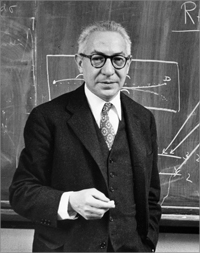
\includegraphics[width = 1.0in]{rabii}
  \end{center}
  \ech
\end{frame}

\begin{frame}\frametitle{\bch 如果矩阵元消失\ech}
  \bch
  矩阵元消失意味着加入振荡的电场时,激发态不会向基态衰变:激发态在电偶极子跃迁的情况下是稳定的。

  但是这并不意味着激发态永远不变,可以存在其他可能的路径。
  \ech
\end{frame}
\begin{frame}\frametitle{\bch 选择定则\ech}
  \bch
  首先,位置算符与自旋无关,这意味着要求
  \be
  \Delta s = \Delta m_s = 0
  \ee
  否则,矩阵元消失。
  \ech
\end{frame}
\begin{frame}\frametitle{\bch 选择定则\ech}
  \bch
  哈密顿量微扰项一部分为$E_z \cdot \langle \psi|z|\psi\rangle$,实际上,利用对易关系$[L_z,z] = 0$,有
  \be
  \langle n^{\prime},l^{\prime}m^{\prime}|[L_z,z]|n,l,m\rangle = \hbar (m^{\prime}-m)\langle n^{\prime},l^{\prime}m^{\prime}|z|n,l,m\rangle
  \ee
  所以只有当$m=m^{\prime}$时,$\langle n^{\prime},l^{\prime}m^{\prime}|z|n,l,m\rangle\ne 0$。故如果电场在$z$轴,当且仅当$\Delta m = 0$时才能发生跃迁。
  \ech
\end{frame}
\begin{frame}\frametitle{\bch 选择定则\ech}
  \bch
  如果电场在$x,y$轴,由对易关系$[L_z,x\pm iy] = \pm \hbar (x\pm iy)$可得
  \be
  \begin{aligned}
  \langle n^{\prime},l^{\prime},m^{\prime}|[L_z,x\pm iy]|n,l,m\rangle &=& \hbar (m^{\prime}-m)\langle n^{\prime},l^{\prime},m^{\prime}|x\pm iy|n,l,m\rangle \\
  &=&\pm\hbar \langle n^{\prime},l^{\prime},m^{\prime}|x\pm iy|n,l,m\rangle
  \end{aligned}
  \ee
  所以只有当
  \be
  \Delta m = \pm 1
  \ee
  矩阵元$ \langle n^{\prime},l^{\prime}m^{\prime}|[L_z,x\pm iy]|n,l,m\rangle$才不为0。故如果波矢在$z$轴,则满足$\Delta m = \pm 1$才能跃迁。
  \ech
\end{frame}
\begin{frame}{\bch 选择定则\ech}
  \bch
  同理,利用对易关系$[L^2,[L^2,\vec{x}]] = 2\hbar^2(\vec{x}L^2+L^2\vec{x})$
  最终可以得到$\Delta l=\pm 1$时,才能发生跃迁。上述推导感觉上很凑巧,一个更加系统地方法是使用 Wigner-Eckart 定理,这个定理基于旋转群的表示论。
  \ech
\end{frame}
\begin{frame}\frametitle{\bch例子\ech}
  \bch
  $2p\rightarrow 1s$     $\tau \simeq 10^{-9}\SIs$

  $2s\rightarrow 1s$     Forbidden, find another route $\tau \simeq 10^{-1} \SIs$

  对于磁偶极子的跃迁,有不同的跃迁规则。氢原子的超精细能级:10 million years!
  \ech
\end{frame}
\section{Spontaneous Emission}
\begin{frame}\frametitle{\bch 自发辐射\ech}
  \bch
  试问在通常的量子力学,如果一个原子处于激发态,把它放在真空中,会发生什么?答案:Nothing Happened. 但是实际上,我们知道它会自发地变为基态,辐射光子。我们说,激发态有一定的寿命$\tau$,这一节我们就来估算$\tau$。

  显然,通常的量子力学解释不了上述现象,完整的解释需要用到量子场论。即我们需要学习光子的量子力学描述,在本讲最后我们会涉及一点。

  但是,如果假设上述现象是成立的,一个聪明的统计力学方法可以帮助我们估算寿命$\tau$,我们下面介绍这个方法。
  \ech
\end{frame}
\begin{frame}\frametitle{\bch 衰变方程\ech}
  \bch
  假设有$N_1$个粒子处于基态上,$N_2$个粒子处于激发态,我们猜测,激发态向基态跃迁的速率(单位时间内跃迁的个数)为$A_{21}$,我们假设有下列关系成立
  \be
  \frac{dN_2}{dt} = -A_{21}N_2
  \ee
  解得$\tau = 1/A_{21}$。然后我们什么也没算出来,这时我们采取一个聪明的方法,将这一大群原子暴露在黑体谱中$\rho (\omega)$。这时,有一部分基态的电子就会跃迁到激发态,因为激发态的概率正比于该频率光子的能量,这个效应引起的速率为$\rho (\omega_0) B_{12}$。又因为我们黑体谱的存在,又会激发激发态的电子跃迁回基态,这个过程叫做受激辐射(stimulated emission),这个效应引起的激发态跃迁回基态的速率为$\rho (\omega_0) B_{21}$
  \ech
\end{frame}
\begin{frame}\frametitle{\bch 爱因斯坦$A,B$系数\ech}
  \bch
  考虑到上述效应,基态和激发态的粒子数目随时间演化的方程改为
  \be
  \begin{aligned}
  \frac{dN_2}{dt} &=& \rho(\omega_0)(B_{12}N_1 - B_{21}N_2) - A_{21}N_2\\
  \frac{dN_1}{dt} &=& -\rho(\omega_0) (B_{12}N_1 - B_{21}N_2) + A_{21}N_2
  \end{aligned}
  \ee
  上面的系数$A_{21},B_{21},B_{12}$被称为爱因斯坦$A,B$系数。
\ech
\end{frame}
\begin{frame}\frametitle{\bch 计算爱因斯坦$A,B$系数\ech}
  \bch
  根据统计力学,在温度$T$下,有
  \be
  \frac{N_2}{N_1} = \frac{g_2}{g_1}\frac{e^{-E_2/k_BT}}{e^{-E_2/k_BT}} = \frac{g_2}{g_1} e^{-\hbar\omega_0/k_BT}
  \ee
  其中$g_1,g_2$为基态和激发态上的兼并态数目。如果达到热平衡(基态和激发态粒子数目保持恒定),则有
  \be
  \rho(\omega_0) = \frac{A_{12} N_2}{B_{12}N_1 - B_{21}N_2}
  \ee
  将上述热力学关系式带入,再利用黑体辐射的普朗克公式,得到
  \be
  \rho(\omega) = \frac{A_{21}}{B_{12}(g_1/g_2)e^{\hbar \omega_0/kT}-b_{12}} = \frac{\hbar}{\pi^2c^3}\frac{\omega^3}{e^{\hbar\omega/k_BT}-1}
  \ee
  \be
  g_1B_{12} = g_2B_{21},\, A_{21} = \frac{\hbar\omega^3}{\pi^2c^3}B_{21}
  \ee
  因此,三个爱因斯坦系数只要计算一个就可以得到另外两个。
\ech
\end{frame}

\begin{frame}\frametitle{\bch 计算爱因斯坦$A,B$系数\ech }
  \bch
  回忆电场较弱时激发态出现的概率
  \be
  P_2(t) \simeq \frac{\Omega^2}{\delta^2} \sin^2\left(\frac{\delta t}{2}\right)
  \ee
  如果假设电场$\vec{E} = (0,0,\varepsilon)$,则有
  \be
  \Omega^2 = \frac{e^2\varepsilon^2}{\hbar^2}|\langle\psi_1|z|\psi_2\rangle|^2
  \ee
  利用$\rho(\omega) =\frac{1}{2}\epsilon_0 E^2$,对于所有的频率积分。
  \be
  P_2(t) = \frac{2e^2}{\epsilon_0 \hbar^2}\langle\psi_1|z|\psi_2\rangle|^2\int d\omega \frac{\rho(\omega)}{(\omega-\omega_0)^2)}\sin^2\left(\frac{(\omega-\omega_0)}{2}t\right)
  \ee
  \ech
\end{frame}

\begin{frame}\frametitle{\bch计算爱因斯坦$A,B$系数\ech }
  \bch
    因为上述积分只在$\omega = \omega_0$处贡献比较大,所以可以作近似$\rho(\omega) = \rho(\omega_0)$,得到
    \be
    P_2(t) = \frac{e^2\pi}{\epsilon \hbar^2}\rho(\omega_0)|\langle\psi_1|z|\psi_2\rangle|^2t
    \ee
    实际上,上面只是得到了一个一阶近似,真正重要的是
    \be
    \dot{P}_2(t) =\frac{e^2\pi}{\epsilon \hbar^2}\rho(\omega_0)|\langle\psi_1|z|\psi_2\rangle|^2
    \ee
    这就是原子对于光的吸收速率。
    最终我们得到了爱因斯坦系数
    \be
    B_{12} = \frac{e^2\pi}{3\epsilon \hbar^2}|\langle\psi_1|\vec{x}|\psi_2\rangle|^2
    \ee
    上面的$1/3$因子是因为考虑了各个方向的缘故。所以当矩阵元越小,激发态生存的时间就越长。
    \ech
  \end{frame}

\section{Toy Model of Photons}
\begin{frame}\frametitle{\bch光子状态的描述\ech}
  \bch
  每一个光子的状态可以由它的动量和偏振来描述。偏振可以分解为两种偏振态(如左旋和右旋),使用$\lambda$来标记$(\lambda = 1,2)$。对于大量的光子,我们对于他们的偏振和动量进行分类,我们数一数对于确定动量和偏振的光子有多少个。故光子的量子态可以记为
  \be
  |\{n_{\vec{k},\lambda}\}\rangle
  \ee
  这样我们就完全描述了一堆光子,没有光子的真空记为$|0\rangle$。对于具有相同动量和偏振的光子,我们无法分辨。
  \ech
\end{frame}
\begin{frame}\frametitle{\bch产生与湮灭算符\ech}
  \bch
  与通常我们研究的粒子不同,光子可以凭空产生,光子数不守恒。受简谐振子的启发,我们对于特定的动量和偏振,引入产生和湮灭算符$a_{\vec{k},\lambda}^{\dagger},a_{\vec{k},\lambda}$,他们满足像谐振子中升降算符一样的对易关系
  \be
     [a_{\vec{k},\lambda},a_{\vec{k}^{\prime},\lambda^{\prime}}^{\dagger}]=\delta_{\vec{k}\vec{k}^{\prime}}\delta_{\lambda\lambda^{\prime}}
  \ee
  因此$ |\{n_{\vec{k},\lambda}\}\rangle$记为
  \be
  |\{n_{\vec{k},\lambda}\}\rangle = \prod_{\vec{k},\lambda} \frac{(a_{\vec{k},\lambda}^{\dagger})^{n_{\vec{k},\lambda}}|0\rangle}{\sqrt{n_{\vec{k},\lambda}!}}
  \ee
  \ech
\end{frame}
\begin{frame}\frametitle{\bch哈密顿量\ech}
  \bch
  因此,光子的哈密顿量为
  \be
  H = \sum_{\vec{k},\lambda} \left(\hbar \omega a_{\vec{k},\lambda}^{\dagger}a_{\vec{k},\lambda}+\frac{1}{2}\right)
  \ee
  由这个哈密顿量实际上可以得到$|\{n_{\vec{k},\lambda}\}\rangle$是本征态,能量的本征值为
  \be
  E = n_{\vec{k},\lambda} \hbar \omega
  \ee
  \ech
\end{frame}
\begin{frame}\frametitle{\bch相干态\ech}
  \bch
  有一种特殊的状态,模拟了经典力学中的谐振子,它是
  \be
  |\alpha\rangle = e^{\alpha a^{\dagger} - \alpha^{*}a} |0\rangle = e^{-|\alpha^2|/2}e^{\alpha a^{\dagger}}|0\rangle
  \ee
  其中参数$\alpha$与总光子数有关
  \be
  n = \langle \alpha |a^{\dagger}a|\alpha\rangle = |\alpha|^2
  \ee
  如何产生这样一个量子态?详见附录。
  \ech
\end{frame}
\begin{frame}\frametitle{\bch 杰恩斯-卡明斯模型\ech}
  \bch
  现在,有了光子的toy model,我们可以研究光子如何与原子相互作用。我们将原子的基态记作$|\downarrow\rangle = (0,1)^{T}$,激发态记作$|\uparrow\rangle = (1,0)^{T}$。因此原子的哈密顿量为
  \be
  H =\frac{1}{2}\hbar \omega_0\left(
  \begin{array}{cc}
    1&0\\0&-1
  \end{array}
  \right)
  \ee
  我们考虑原子的周围有一群光子,光子的状态和哈密顿量为(略去下标)
  \bea
  |n\rangle &=& \frac{(a^{\dagger})^n}{\sqrt{n!}}|0\rangle\\
  H &=& \hbar \omega (a^{\dagger}a+1/2)
  \eea
  \ech
\end{frame}
\begin{frame}{\bch 杰恩斯-卡明斯模型\ech}
  \bch
  将原子的希尔伯特空间和光子的希尔伯特空间做直积
  \be
  \mathcal{H} = \mathcal{H}_{\rm atom} \bigotimes \mathcal{H}_{\rm photons}
  \ee
  例如,具有$n$个光子且原子处于激发态就表示为$|n;\uparrow\rangle$。为了描述光子和原子作用,哈密顿量为
  \be
  H_{JC} = \frac{\hbar}{2} \left(
  \begin{array}{cc}
    \omega_0 & ga \\
    ga^{\dagger} & -\omega_0
  \end{array}
  \right)
  +\hbar\omega a^{\dagger} a
  \ee
  其中$g$表征光子和原子的耦合。上面的哈密顿量又被称作杰恩斯-卡明斯(Jaynes-Cummings)模型。
  \ech
\end{frame}
\begin{frame}{\bch 思考题\ech}
  \bch
    \be
  H_{JC} = \frac{\hbar}{2} \left(
  \begin{array}{cc}
    \omega_0 & ga \\ ga^{\dagger} & -\omega_0 \end{array}\right)
  +\hbar\omega a^{\dagger} a
  \ee
  这个哈密顿量如何与态$|n-1;\uparrow\rangle$作用?
  \ech
  \begin{center}

\includegraphics[width = 1.2in]{not_understand.jpg}
\end{center}
\end{frame}
\begin{frame}\frametitle{\bch 计算矩阵元\ech}
  \bch
  我们研究从状态$|n-1;\uparrow\rangle$到状态$|n;\downarrow\rangle$的演化,为此我们要计算上面哈密顿量的矩阵元。计算结果为
  \be
  H_n =\left(
  \begin{array}{cc}
    (n-1)\omega+\frac{1}{2}\omega_0 &\frac{1}{2}g\sqrt{n} \\
    \frac{1}{2}g\sqrt{n} & n\omega - \frac{1}{2} \omega_0
  \end{array}
  \right)
  \ee
  这意味着原子的基态和激发态并不是这个哈密顿量的本征态,经过计算,能量的本征值为
  \be
  E_{\pm} = \left( n+ \frac{1}{2}\right) \hbar \omega \pm \frac{1}{2}\hbar\sqrt{g^2n+\delta^2}
  \ee
  本征态为
  \bea
  |n_+\rangle &=& \sin\theta |n-1;\uparrow\rangle-\cos\theta|n;\downarrow\rangle \\
  |n_-\rangle &=& \cos\theta |n-1;\uparrow\rangle+\sin\theta|n;\downarrow\rangle 
  \eea
  其中$\tan(2\theta) = \frac{g\sqrt{n}}{\delta},\, \delta = \omega_0-\omega$。
  \ech
\end{frame}
\begin{frame}\frametitle{\bch 再论拉比进动\ech}
  \bch
  初始情况,原子处于基态$|\Psi (t=0)\rangle =|n,\downarrow\rangle = \sin\theta|n_-\rangle - \cos\theta|n_+\rangle$,之后开始演化
  \be
  |\Psi (t)\rangle =e^{-iE_-t/\hbar}\sin\theta|n_-\rangle -e^{-iE_+t/\hbar} \cos\theta|n_+\rangle
  \ee
  计算得到激发态的概率为
  \be
  P_\uparrow (t)= \frac{g^2n}{g^2n + \delta^2} \sin^2 \left(\frac{\sqrt{g^2n+\delta^2}t}{2}\right)
  \ee
  这与前面得到的结果相同,拉比频率$\Omega = g\sqrt{n}$。
  \ech
\end{frame}
\begin{frame}\frametitle{\bch再论拉比进动\ech}
  \bch
  这次,我们将周围的光子换成相干态的光子(激光)
  \be
  |\Psi\rangle = e^{-|\alpha|^2/2}e^{\alpha a^{\dagger}}|0,\downarrow\rangle = e^{-|\alpha|^2/2}\sum_{n=0}^{\infty} \frac{\alpha^n}{\sqrt{n!}} |n,\downarrow\rangle
  \ee
  考虑相干态中有大量的光子$|\alpha|\gg 1$,通过同样地方法求态的演化,可以得到激发态的概率
  \be
  P_{\uparrow}(t) = e^{-|\alpha|^2}\sum_{n=0}^{\infty} \frac{|\alpha|^{2n}}{n!}\sin^2\left(\frac{g\sqrt{n}t}{2}\right)
  \ee
  \ech
\end{frame}
\begin{frame}\frametitle{\bch 死亡与复生\ech}
  \bch
  激发态概率
  \be
  P_{\uparrow}(t) = \frac{1}{2}-\frac{1}{2}e^{-|\alpha|^2}\sum_{n=0}^{\infty} \frac{|\alpha|^{2n}}{n!}\cos\left(g\sqrt{n}t\right)
  \ee
  考察系数$\frac{|\alpha|^{2n}}{n!}$,取对数并利用斯特林公式
  \be
  \ln\frac{|\alpha|^{2n}}{n!} \simeq 2n\ln |\alpha| - n\ln n +n
  \ee
  由此可知,当$n = |\alpha|^2$时上面的系数有最大值。我们将其在极大值附近泰勒展开到二阶
  \be
  \frac{|\alpha|^{2n}}{n!} \simeq \frac{1}{2\pi |\alpha|^2} e^{|\alpha|^2 - m^2/2|\alpha^2|}
  \ee
  其中$m = n-|\alpha|^2$。如果$|\alpha|^2$充分大,求和可以从$-\infty$到$\infty$。
  \ech
\end{frame}
\begin{frame}\frametitle{\bch 死亡与复生\ech}
  \bch
  所以我们有
  \be
  P_{\uparrow}(t) = \frac{1}{2}-\frac{1}{2}\sum_{m=-\infty}^{\infty}  e^{- m^2/2|\alpha^2|}\cos(gt\sqrt{|\alpha^2|+m})
  \ee
  画出来如下图所示。
  \cpic{0.2}{resurrection}
  \ech
\end{frame}
\begin{frame}\frametitle{\bch 死亡与复生\ech}
  \bch
  不断地沉默与复生,直到最后出现不稳定的波动。
  \cpic{0.3}{overall}
  \ech
\end{frame}
\begin{frame}\frametitle{\bch 总结\ech}
 \bch
 能发出光来就不错了。
 \cpic{0.3}{drop_school}
  \ech
\end{frame}
\section{Appendix}
\begin{frame}\frametitle{\bch 附录:如何产生相干态\ech}
  \bch
  我们来说明,下面的哈密顿量可以产生相干态
  \be
  H = \hbar \omega\left(a^{\dagger}a+\frac{1}{2}\right) + \hbar(f^{*}(t)a+f(t) a^{\dagger})
  \ee
  \ech
\end{frame}
\begin{frame}\frametitle{\bch相互作用绘景\ech}
  \bch
  求解这个哈密顿量几乎不可能,我们借助于相互作用绘景。相互作用绘景将哈密顿量分解成两项$H = H_0 +H_I$,其中$H_0$一般是我们熟知的系统,而$H_I$是对于系统的微扰。相互作用绘景中,态矢和算符的定义为
  \bea
  |\psi\rangle_I &=& e^{iH_0 t} |\psi\rangle_S \\
  \mathcal{A}_I &=& e^{iH_0 t}\mathcal{A}_S e^{-iH_0 t}
  \eea
  从薛定谔绘景的算符和态矢演化方程出发,可以得到相互作用绘景态矢和算符的演化方程
  \bea
  i\hbar \frac{d|\psi\rangle}{dt} &=& H_I |\psi\rangle \\
  \frac{d\mathcal{A}}{dt} &=& \frac{i}{\hbar}[H,\mathcal{A}]
  \eea
  可以证明,不论在哪个绘景,矩阵元$\langle \psi_1|\mathcal{A}|\psi_2\rangle$相同。
  \ech
\end{frame}
\begin{frame}\frametitle{\bch 时间演化算符\ech}
  \bch
  首先求得$H_I$在相互作用绘景中的形式,根据定义
  \be
  H_I = \hbar e^{iH_0 t/\hbar}(f^{*}(t)a+f(t) a^{\dagger})e^{-iH_0 t/\hbar} = \hbar\left( e^{-i\omega t} f^{*}(t)a+e^{i\omega t}f(t)a^{\dagger}\right)
  \ee
  由演化算符的方程
  \be
  i\hbar \frac{\partial U_I}{\partial t} = H_I U_I
  \ee
  得到解是
  \be
  U_I(t) = \exp \left(\alpha(t)a^{\dagger} - \alpha^{*}a+i\varphi(t)\right)
  \ee
  其中$\alpha = -i \int dt^{\prime}f(t^{\prime})e^{i\omega t^{\prime}},\, \varphi(t) = \frac{1}{2}\int dt^{\prime}{\rm Im}(\dot{\alpha}^{*}\alpha)$。
  \ech
\end{frame}
\begin{frame}\frametitle{\bch 构造相干态\ech}
  \bch
  如果取$f(t) = f_0 e^{-i\omega t}$,就得到了我们要的相干态。
  \ech
\end{frame}

  
\end{document}
